\documentclass[11pt, oneside]{article}   	% use "amsart" instead of "article" for AMSLaTeX format
\usepackage{geometry}                		% See geometry.pdf to learn the layout options. There are lots.
\geometry{letterpaper}                   		% ... or a4paper or a5paper or ... 
%\geometry{landscape}                		% Activate for rotated page geometry
%\usepackage[parfill]{parskip}    		% Activate to begin paragraphs with an empty line rather than an indent
\usepackage{graphicx}				% Use pdf, png, jpg, or eps§ with pdflatex; use eps in DVI mode
								% TeX will automatically convert eps --> pdf in pdflatex		
\usepackage{epstopdf}
\usepackage{amssymb}
\usepackage[pdf]{pstricks}
\usepackage{subfig}
\usepackage[colorlinks]{hyperref}
\usepackage[sort&compress]{natbib}
\usepackage{listings}
\title{Example of Stata-Generated Tables and Natlib References}
\author{Pierre-Carl Michaud \\ HEC Montreal}

\begin{document}
\maketitle

\section{Summary Stats}

\subsection{Estout package}

The stats are produced here in Table \ref{tab:desc-estout}

\begin{table}[htp]
  \centering
  {
\def\sym#1{\ifmmode^{#1}\else\(^{#1}\)\fi}
\begin{tabular}{l*{2}{c}}
\hline\hline
            &\multicolumn{1}{c}{female}&\multicolumn{1}{c}{male}\\
\hline
age         &       49.02         &       49.52         \\
            &     (29.05)         &     (28.73)         \\
[1em]
income      &    31991.15         &    35049.33         \\
            &   (93980.1)         &  (118056.4)         \\
\hline
\(N\)       &        5057         &        4943         \\
\hline\hline
\end{tabular}
}

  \caption{Descriptive Statistics by Gender}
  \label{tab:desc-estout}
\end{table}

\subsection{Brut Force}
The descriptive statistics you asked are reproduced in Table \ref{tab:desc}. 

\begin{table}[htp]
\centering
\begin{tabular}{lrrrr} 
\hline \hline  & mean ($\mu$) & sd ($\sigma$) & min & max \\
Age &  49.266 &  28.894 &   0.000 &  99.000 \\
Gender &   0.494 &   0.500 &   0.000 &   1.000 \\
Household Income &  3.4e+04 &  1.1e+05 &  24.730 &  3.3e+06 \\
\hline \hline \end{tabular}

\caption{Descriptive Statistics from Estimation Sample}
\label{tab:desc}
\end{table}

You should know that \citep{lusardi_financial_2007} found exactly the same thing. Other studies have found the same thing \citet{Lusardi2017OptimalInequality}. Just like what \citet{Card1990TheMarket}.

\begin{table}[!htp]
\centering
\begin{tabular}{lc}
\hline\hline
 Parameter   & Value  \\
Risk aversion ($\sigma$)     & 3.0 \\
\hline\hline
\end{tabular}
\caption{Calibrated Parameters}
\end{table}


The stata code is reproduced in the appendix (See Listing \ref{lst:stata}). 

\section{Regression Tables}

\begin{table}[htp]
  \centering
  {
\def\sym#1{\ifmmode^{#1}\else\(^{#1}\)\fi}
\begin{tabular}{l*{2}{c}}
\hline\hline
            &\multicolumn{1}{c}{female}&\multicolumn{1}{c}{male}\\
\hline
age         &       33.12         &      -155.2\sym{**} \\
            &     (45.50)         &     (58.41)         \\
[1em]
\_cons      &     30367.5\sym{***}&     42731.8\sym{***}\\
            &    (2592.6)         &    (3343.8)         \\
\hline
\(N\)       &        5057         &        4943         \\
adj. \(R^{2}\)&      -0.000         &       0.001         \\
\hline\hline
\end{tabular}
}

  \caption{Regression Estimates by Gender}
  \label{tab:reg-gender}
\end{table}

\section{Figures}

Adding a figure such as Figure \ref{fig:scatter} is simple. 

\begin{figure}[htp]
    \centering
    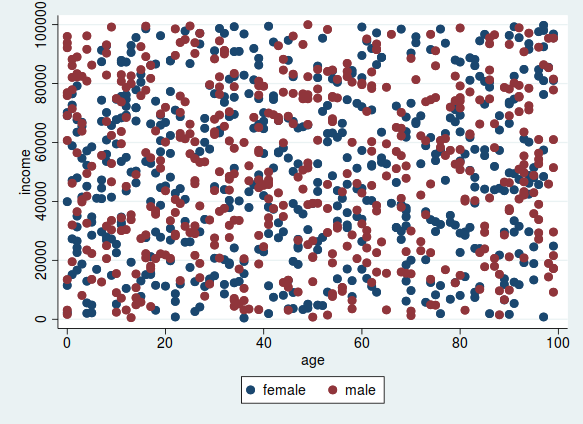
\includegraphics[scale=0.5]{test.png}
    \caption{Relationship between Age and Income by Gender}
    \label{fig:scatter}
\end{figure}

\bibliography{references}
\bibliographystyle{apalike}%{plainnat} %{plain-annote}

\newpage

\appendix

\section*{Appendix: Stata Code}
\lstinputlisting[basicstyle=\tiny,label=lst:stata, frame=single,caption=Contents of test.do,captionpos=b]{test.do}

\end{document}
